\documentclass[a4paper,twoside,12pt]{article}
%\usepackage [reqno] {amsmath}
\usepackage{amsfonts,amstext}
\usepackage{amsmath}
\usepackage{german}
\usepackage{graphicx}
\usepackage{fullpage}

\newcommand{\ZETTELNUMMER}{4}

\newcounter{AUFGNR}
\setcounter{AUFGNR}{1}
\newcommand{\AUFGABE}[2]{\vspace{0.3cm}\item[Aufgabe~\arabic{AUFGNR}]\stepcounter{AUFGNR} #1\hfill\emph{#2}}


\newcommand{\floor}[1]{\left\lfloor{#1}\right\rfloor}
\newcommand{\ceil}[1]{\left\lceil{#1}\right\rceil}
\newcommand{\half}[1]{\frac{#1}{2}}
\newcommand{\N}{\mathbb{N}}



\renewcommand{\labelenumi}{(\alph{enumi})}
\renewcommand{\labelenumii}{(\roman{enumii})}


\begin{document}
\pagestyle{empty}
\hrule\medskip
\rule{0ex}{0ex}\\[-1ex]
\ZETTELNUMMER. Aufgabenblatt zur Vorlesung

\smallskip
\noindent
\large
\textbf{Nichtsequentielle und Verteilte Programmierung}\hfill SoSe
2018 \\[0.5ex]
\normalsize
Anton Oehler, Mark Niehues

\newcommand{\immer}{\Box}
\newcommand{\irgendwann}{\lozenge}
\newcommand{\folgt}{\Rightarrow}
\newcommand{\oder}{\vee}
\newcommand{\und}{\wedge}

\medskip\hrule

\begin{description}
% Aufgabe 1
\AUFGABE{Lineare Temporale Logik I}{10 Punkte}
\begin{enumerate}
  \item { \[
     \lozenge \Box\, p \Leftrightarrow \Box \lozenge\, p
  \]}
  
  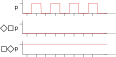
\includegraphics[width=0.5\textwidth]{1_a.png}
  
Anhand der Grafik lässt sich erkennen, dass die Aussage nicht für alle Belegungen gilt.

  \item \begin{eqnarray}
		     ((\Box\, p \Rightarrow \lozenge\, q) \land \lozenge \Box\, q )& \Rightarrow & \lozenge\, q \\
		     ((\neg \Box\, p \lor \lozenge\, q) \land \lozenge \Box\, q )& \Rightarrow & \lozenge\, q
		\end{eqnarray}

\item 
\begin{enumerate}
\item zu Zeigen: $(\Box\, p \wedge \Box\, q) \Leftrightarrow \Box (p \wedge q)$

$
\Box\, p_i \wedge \Box\, q_i := \forall j \geq i : p_j \wedge \forall j \geq i:q_j => \forall j \geq i: p_j \wedge q_j
$

$
\Box (p_i \wedge q_i) := \forall j \geq i: p_j \wedge q_j
$ 

q.e.d.

\item zu Zeigen: $(\lozenge\, p \vee \lozenge\, q) \Leftrightarrow \lozenge (p \vee q)$

$
\lozenge\, p_i \vee \lozenge\, q_i := \exists j \geq i: p_j \vee \exists j \geq i: q_j => \exists j \geq i: p \vee q
$

$
\lozenge (p \vee q) := \exists j \geq i: p \vee q
$

q.e.d.
\end{enumerate}
\end{enumerate}

% Aufgabe 2
\AUFGABE{Lineare Temporale Logik II}{10 Punkte}
\begin{enumerate}
\item
\begin{enumerate}
\item
$I_x(\alpha U \beta) = I_x(\alpha )\dot{U} I_x(\beta)$ mit $\dot{U}: \{t,f\}^{N x N} \rightarrow \{t,f\}^N$ \\
wobei $\dot{U}((a_i)_{i\in N}, (b_i)_{i\in N}) = (w_i)_{i\in N}$\\
und $w_i = \begin{cases} t & falls\, \exists j\geq i: b_j = t \land \forall k\in [i, ..., j): a_k = t \\ f & sonst \end{cases}$
\begin{figure}
  \includegraphics[width=0.5\textwidth]{2_a_1.png}
\caption{Beispiel für den \textit{bis} Operator}
\end{figure}  

\item
$I_x(\bigcirc \alpha) = \dot{\bigcirc} I_x(\alpha )$ mit $\dot{\bigcirc}: \{t,f\}^N \rightarrow \{t,f\}^N$ \\
wobei $\dot{\bigcirc}((a_i)_{i\in N}) = (w_i)_{i\in N}$\\
und $w_i = \begin{cases}
 t, & falls\, a_{i+1} = t\\
 f, & sonst 
 \end{cases}$  
 	\begin{figure}
 	   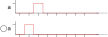
\includegraphics[width=0.5\textwidth]{2_a_2.png}
	\caption{Beispiel für den \textit{nächster} Operator}
 	\end{figure}

\end{enumerate}

\item 
Falls mehrere Threads im Spiel sind, ist der nächste Schritt unter Annahme schwacher Fairness nicht genau definiert.

\item
$ \Box\, a = aUa \land \neg (aU\neg a)$\\
$ \lozenge\, a = aUa \lor \neg aUa$\\

\end{enumerate}

% Aufgabe 1
\AUFGABE{Der Algorthmus von Peterson II}{10 Punkte}
\begin{verbatim}
======================================================
  global adrin = false, bdrin = false, letzter = a
a1: U                     | b1: U
a2: adrin  <- true        | b2: bdrin  <- true
a3: letzter <- a          | b3: letzter <- b
a4: while bdrin &&        | b4: while adrin &&
          letzter = a do  |           letzter = b do
a5:     NOP               | b5:     NOP
a6: K                     | b6: K
a7: adrin <- false        | b7: bdrin <- false
\end{verbatim}
F"ur alle m"oglichen Zustandsfolgen gilt:
\begin{itemize}
	\item $\immer(a_1 \folgt \irgendwann (a_2 \oder a_\bot))$
	\item $\immer(a_2 \folgt \irgendwann a_3)$
	\item $\immer(a_3 \folgt \irgendwann a_4)$
	\item $\immer(a_4 \folgt \irgendwann (a_5 \oder a_6)$
	\item $\immer(a_5 \folgt \irgendwann a_4)$
	\item $\immer(a_6 \folgt \irgendwann a_7)$
	\item $\immer(a_7 \folgt \irgendwann a_1)$
	\item $\immer(a_\bot \folgt \immer a_\bot)$
	\item Analog f"ur die Zust"ande von $b$
\end{itemize}

Au"serdem legen wir folgende Invarianten fest:
\begin{itemize}
	\item $\immer(letzter = a \oder letzter = b)$
	\item $\immer(adrin \equiv a_3 \oder a_4 \oder a_5 \oder a_6 \oder a_7)$
	\item $\immer(bdrin \equiv b_3 \oder b_4 \oder b_5 \oder b_6 \oder b_7)$
	% \item $\immer(adrin \und bdrin \equiv
\end{itemize}

\begin{enumerate}
	\item Zu beweisen:
	\begin{itemize}
		\item $(a_6 \und (b_4 \oder b_5)) \folgt (adrin \und letzter = b)$
		\item $((a_4 \oder a_5) \und b_6) \folgt (bdrin \und letzter = a)$
	\end{itemize}
	\item Zu zeigen:
	\begin{itemize}
		\item $\immer \big [(a_4 \und \immer \neg a_6) \folgt \immer \irgendwann (bdrin \und letzter \neq b) \big ]$
		\item $\immer \big [\irgendwann \immer (\neg bdrin) \oder \irgendwann (letzter = b) \big]$
		\item $\immer \big [(a_4 \und \immer \neg a_6 \und \irgendwann (letzter = b)) \folgt \irgendwann \immer (letzter = b)) \big ]$
	\end{itemize}
\end{enumerate}

\end{description}
\end{document}